%\documentclass[10pt]{beamer}
\documentclass[aspectratio=169]{beamer}

\usetheme[progressbar=frametitle]{metropolis}
\usepackage{appendixnumberbeamer}

\usepackage{booktabs}
\usepackage[scale=2]{ccicons}

\usepackage{biblatex}
  \addbibresource{type_talk.bib}
\usepackage{minted}
\usepackage{array}
\usepackage{tabularx}
\usepackage{makecell}
\usepackage{svg}

\usepackage{xspace}
\newcommand{\themename}{\textbf{\textsc{metropolis}}\xspace}

\usepackage{pgfpages}
% These slides also contain speaker notes. You can print just the slides,
% just the notes, or both, depending on the setting below. Comment out the want
% you want.
\setbeameroption{hide notes} % Only slide
%\setbeameroption{show only notes} % Only notes
%\setbeameroption{show notes on second screen=right} % Both

\title{PHP's Type System Dissected}
\subtitle{Understanding how PHP's type system works}
\date{\today}
%\date{14 Octobre 2022}
%\email{<girgias@php.net>}
\author{George Peter Banyard}
\institute{The PHP Foundation}

% Logo only on title page
%\titlegraphic{\includegraphics[width=.2\textwidth]{forumphp-2022.png}}
\titlegraphic{
    %\includesvg[inkscapelatex=false,width=0.25\columnwidth]{images/php_foundation.svg}
    %\hfill
    % \baselineskip is the "height" of one line (The normal vertical distance between lines in a paragraph.)
    
    \includesvg[inkscapelatex=false,height=4\baselineskip]{images/conf_logo.svg}
    %
\includegraphics[height=4\baselineskip]{images/icon_php_london.png}
}

%TODO Improve title page to not overflow vertically ideally.
\makeatletter
\setbeamertemplate{title page}{
  \begin{minipage}[b][\paperheight]{\textwidth}
    \vfill%
    \ifx\inserttitle\@empty\else\usebeamertemplate*{title}\fi
    \ifx\insertsubtitle\@empty\else\usebeamertemplate*{subtitle}\fi
    \usebeamertemplate*{title separator}
      \begin{columns}[T,onlytextwidth]
        \column{0.5\textwidth}
            \ifx\beamer@shortauthor\@empty\else\usebeamertemplate*{author}\fi
            \ifx\insertdate\@empty\else\usebeamertemplate*{date}\fi
            \ifx\insertinstitute\@empty\else\usebeamertemplate*{institute}\fi
        \column{0.5\textwidth}
            %\vfill
            \vspace{0.5cm}
            \hfill
            \ifx\inserttitlegraphic\@empty\else\inserttitlegraphic\fi
            %\hfill
            %\vfill
      \end{columns}
    \vfill
    \vspace*{1cm}
  \end{minipage}
}
\makeatother
% Logo on every slide
%\logo{\includegraphics[width=3cm]{forumphp-2022.png}}
\newcommand{\descriptionsize}{Type universel $\top$ :}

\newcommand{\union}{\:\mathrel{|}\:}
\newcommand{\inter}{\mathrel{\&}}
\newcommand{\mif}{\text{ if }}
\newcommand{\subtype}{\mathrel{<:}}
\newcommand{\suptype}{\mathrel{:>}}
\newcommand{\subtypenot}{\ \not\!\!\subtype}
\newcommand{\type}[1]{\texttt{\textbf{#1}}}

\definecolor{AFUP}{HTML}{36a7df}
\definecolor{AFUP_text}{HTML}{1d2241}
\begin{document}

\maketitle

\begin{frame}{About me}
    \begin{center}
    \begin{columns}[T]
        \column{0.5\paperwidth}
            \begin{description}
                \item[Mastodon:] @Girgias@phpc.social
                \item[Twitter:] @Girgias
                \item[GitHub:] Girgias
                \item[Site:] \url{https://gpb.moe}
            \end{description}
            \begin{center}
                \includesvg[inkscapelatex=false,width=0.4\columnwidth]{images/php_foundation.svg}  
            \end{center}
            
        \column{0.5\textwidth}
            \begin{itemize}
                \item Studied pure mathematics
                \item PHP Core dev financed part-time by \alert{The PHP Foundation}
                \item Lead maintainer for the French documentation of PHP
                \item Cares about the type system
                    \cite{banyard_pure_2021}
                    \cite{banyard_disjunctive_2022}
                    \cite{banyard_allow_2022}
                    \cite{banyard_add_2022}
                \item Cares about PHP semantics
                    \cite{banyard_saner_2020}
                    \cite{banyard_saner_2023}
                    \cite{banyard_path_2022}
            \end{itemize}
    \end{columns}
    \end{center}
\end{frame}

\begin{frame}{Table of Contents}
  \setbeamertemplate{section in toc}[sections numbered]
  \tableofcontents%[hideallsubsections]
\end{frame}

%\section[Intro]{Introduction}
%\begin{verbatim}The theme provides sensible defaults to \emph{emphasize} text, \alert{accent} parts or show \textbf{bold} results.\end{verbatim}
%\begin{center}becomes\end{center}

\section{PHP's Type System}
\begin{frame}{What is a type system?}
  \begin{quote}
    A \alert{type system} is a logical system comprising a set of rules that assigns a property called a \textbf{type} to every "term".

    A type system dictates the \textbf{operations} that can be performed on a term.
    \cite{noauthor_type_2022}
    % Ref https://en.wikipedia.org/wiki/Type_system
  \end{quote}
  \note[item]{
    A \alert{type system} is a logical system comprising a set of rules that assigns a property called a \textbf{type} to every "term" (a word, phrase, or other set of symbols). Usually the terms are various constructs of a computer program, such as variables, expressions, functions, or modules.
    A type system dictates the \textbf{operations} that can be performed on a term. For variables, the type system determines the allowed values of that term.
  }
\end{frame}

\begin{frame}{PHP's Type System}
    \note[item]{
        In PHP, a parameter of a function, the return value of a function, or the property of a class can define a type.
    }
    
    The available types are:
    \begin{itemize}
        \item Primitive types
        \item User defined types
        \item Literal types
        \item The \type{callable} type
        \item Composite types
        \item Type aliases
    \end{itemize}
\end{frame}

%\subsection{Base types}
\begin{frame}{Primitive types}
    \begin{description}[\descriptionsize]
     \item[Universal type] \type{mixed} (PHP 8.0)
     \item[Resource type]
     \item[Object type] \type{object} (PHP 7.2)
     \item[Hash table type] \type{array}
     \item[Scalar types] \type{bool}, \type{int}, \type{float}, \type{string}
     \item[Unit type] \type{null} (PHP 8.0*)
     \item[Empty type]  \type{never} (PHP 8.1)
    \end{description}
    And a special return only type:
    \begin{description}[\descriptionsize]
     \item[] \type{void} (PHP 7.1)
    \end{description}
\end{frame}

\begin{frame}{User Defined Types}
    Also called \alert{class-types}, they are:
    \begin{description}[\descriptionsize]
        \item [Interfaces]
        \item [Classes]
        \item [Enumerations] (PHP 8.1)
    \end{description}
    
    Relative class types:
    \begin{description}[\descriptionsize]
        \item [\type{self}]
        \item [\type{parent}]
        \item [\type{static}] (PHP 8.0 as a return type only)
    \end{description}
\end{frame}
\begin{frame}{Literal types}
    A literal type is a concrete subtype of a type, i.e. a value of a type.
    \begin{itemize}
        \item \type{false} (PHP 8.0*)
        \item \type{true} (PHP 8.2)
    \end{itemize}
    \only
    \begin{alertblock}{Warning}
        It's impossible to define a literal type in userland.
        Create an enumeration instead.
    \end{alertblock}
\end{frame}
\begin{frame}{The \type{callable} type}
    Type which represents a function:
    \begin{itemize}
        \item A string of characters: \texttt{"strlen"}
        \item An object/method pair: \texttt{[\$instance, "method"]}
        \item An object which implements \texttt{\_\_invoke()}
        \item A Closure, obtainable with the syntax: \texttt{strlen(...)} (PHP 8.1)
    \end{itemize}

    \begin{alertblock}{Warning}
        It's impossible to define a class property as \type{callable}
    \end{alertblock}
\end{frame}

%\subsection{Composite types}
\begin{frame}{Composites types}
    A composite type is a type composing multiple other types.
    \begin{description}[Simple union type:]
     \item[Intersection type:] \type{A\&B} (PHP 8.1)
     \item[Simple union type:] \type{T|U} (PHP 8.0)
     \item[DNF type:] \type{(X\&Y)|(V\&W)} (PHP 8.2)
    \end{description}
    \begin{block}{Disjunctive normal form}
        In boolean logic, a \alert{Disjunctive Normal Form} or \alert{DNF} is a canonical normal form of a logical formula consisting of a disjunction of conjunctions; it can also be described as an \emph{OR} of \emph{AND}s.
        \cite{noauthor_disjunctive_2022}
        % https://en.wikipedia.org/wiki/Disjunctive_normal_form
    \end{block}
\end{frame}
\begin{frame}{Composites types: why do we care?}
\begin{center}
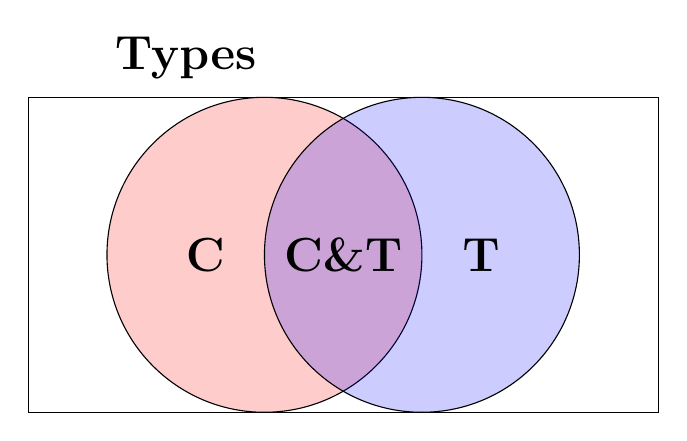
\begin{tikzpicture}
%% You can adjust the opacity here. For venn diagrams it is convenient to have a low opacity so that you can see intersections
	\begin{scope} [fill opacity = .2]
%% The draw command knows a lot of shapes. To make a rectangle you just need to specify two diagonal corners. Make sure you always have a semicolon at the end of your draw commands, otherwise latex flips out.
    \draw (-4,4) rectangle (4,0);
%% Similarly, you can make a circle by specifying the center and then the radius. You can also add a fill color, but if you're printing in black and white you'll probably want to remove that line.
    \draw[fill=red, draw = black] (-1,2) circle (2);
    \draw[fill=blue, draw = black] (1,2) circle (2);
%% We can use the node command to label points. If you put your cursor on "LARGE" or "textbf" a box will drop down with size and text style options.
    \node[opacity=1] at (-2,4.5) {\LARGE\textbf{Types}};
    \node[opacity=1] at (-1.75,2) {\LARGE\textbf{C}};
    \node[opacity=1] at (1.75,2) {\LARGE\textbf{T}};
    \node[opacity=1] at (0,2) {\LARGE\textbf{C\&T}};
    \end{scope}
%% And now you have a venn diagram. Yay!
%\draw[help lines](-5,5) grid (5,-6);    This line can draw the grid lines to help guide you. I use these when I'm writing the code and then delete this line when I publish the pdf.
\end{tikzpicture}
\end{center}
\end{frame}
\begin{frame}{Composites types: why do we care?}
    \textbf{intersection} of types gives us access to \alert{every} API provided by each type

    \textbf{union} of types gives us access \alert{only} to the common API between each type
\end{frame}

\begin{frame}{Type Alias}
    As of PHP 8.2, \type{iterable} type alias resolved at compile time.

    \begin{displaymath}
        \text{\texttt{iterable}} := \text{\texttt{Traversable}}|\text{\texttt{array}} 
    \end{displaymath}

    Before it was a pseudo primitive type.
    
    \begin{alertblock}{Warning}
        It's impossible to define a type alias in userland.
    \end{alertblock}
\end{frame}

\begin{frame}[fragile]{Values are Zvals}
\begin{center}
    \begin{columns}
        \column{0.5\textwidth}
        \begin{minted}[fontsize=\small]{c}
struct _zval_struct {
    zend_value value;
    uint32_t type_info;
};
        \end{minted}

        \column{0.5\textwidth}
        \begin{minted}[fontsize=\small]{c}
#define IS_NULL      1
#define IS_FALSE     2
#define IS_TRUE      3
#define IS_LONG      4
#define IS_DOUBLE    5
#define IS_STRING    6
#define IS_ARRAY     7
#define IS_OBJECT    8
#define IS_RESOURCE  9
/* ... */
        \end{minted}
    \end{columns}
\end{center}
\end{frame}

\begin{frame}[fragile]{zend\_type the internal representation of a type}
    The type of a parameter, return value, or property is represented by a \alert{zend\_type}.
    \begin{minted}[fontsize=\small]{c}
typedef struct {
    void *ptr;
    uint32_t type_mask; // Bit-mask of primitive types
} zend_type;
    \end{minted}
    \texttt{\textbf{ptr}} is either a class name as a string, or a list of types:
    \begin{minted}[fontsize=\small]{c}
typedef struct {
    uint32_t num_types;
    zend_type types[1];
} zend_type_list;
    \end{minted}
\end{frame}

\section{Subtyping and Liskov Substitution Principle}

\begin{frame}{What is a subtyping?}
  \begin{quote}
    In programming language theory, \alert{subtyping} is a form of type polymorphism in which a subtype is a datatype that is related to another datatype (the supertype) by some notion of substitutability.

    \note[item]{
        In programming language theory, subtyping (also subtype polymorphism or inclusion polymorphism) is a form of type polymorphism in which a subtype is a datatype that is related to another datatype (the supertype) by some notion of substitutability, meaning that program elements, typically subroutines or functions, written to operate on elements of the supertype can also operate on elements of the subtype.
    }

    If $S$ is a subtype of $T$, the subtyping relation (written as $S \subtype T$, $S \sqsubseteq T$, or  $S \leq: T$ ) means that any term of type $S$ can \alert{safely} be used in \alert{any} context where a term of type $T$ is expected.
    \note[item]{
        The precise semantics of subtyping here crucially depends on the particulars of how "safely be used" and "any context" are defined by a given type formalism or programming language. The type system of a programming language essentially defines its own subtyping relation, which may well be trivial, should the language support no (or very little) conversion mechanisms.
    }
    \note[item]{
        Due to the subtyping relation, a term may belong to more than one type. Subtyping is therefore a form of type polymorphism. In object-oriented programming the term 'polymorphism' is commonly used to refer solely to this subtype polymorphism, while the techniques of parametric polymorphism would be considered generic programming. 
    }
    \cite{noauthor_subtyping_2022}
    % Ref https://en.wikipedia.org/wiki/Subtyping
  \end{quote}
\end{frame}

\begin{frame}{Liskov Substitution Principle}
    The Liskov Substitution Principle or \alert{LSP} is a particular definition of a subtyping relation, called strong behavioural subtyping.
    It was formulated by Barbara Liskov and Jeannette Wing in 1994. \cite{liskov_behavioral_1994}
    
    The succinct formulation is:
    \begin{quote}
        Let $\mathbf{\phi(x)}$ be a property provable about objects $\mathbf{x}$ of type $\mathbf{T}$. Then $\mathbf{\phi(y)}$ should be true for objects $\mathbf{y}$ of type $\mathbf{S}$ where $\mathbf{S}$ is a subtype of $\mathbf{T}$.
        %Cite https://dl.acm.org/doi/10.1145/197320.197383
    \end{quote}
\end{frame}
\begin{frame}{Liskov Substitution Principle: Simplified}
    LSP is a principle about the replacement of a type with another such that the interactions before and after are not affected.

    \begin{description}[Post-conditions]
        \item[Pre-conditions] cannot be strengthened in the subtype
        \item[Post-conditions] cannot be weakened in the subtype
        \item[Invariants] must be preserved in the subtype
        \note[item]{
            Invariants are stuff like immutable properties, which doesn't mean one cannot add \emph{other} mutable properties in a subtype
        }
        \item[History rule] constraints must be preserved in the subtype
        \note[item]{
            The History Rule is also redefined as an extension map.

            As in any new methods that mutate the state of the supertype \emph{must} be producable by using existing methods on the supertype.
            
            Contraints relate to states of the supertypes only, and not to any additional behaviour   
        }
    \end{description}
\end{frame}
\begin{frame}{Liskov Substitution Principle: Visualized}
    \begin{figure}
    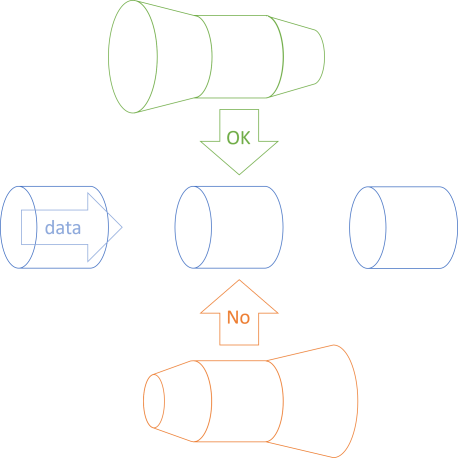
\includegraphics[height=0.75\paperheight]{lsp-pipes.png}
    \caption{
        Visualization of Liskov Substitution Principle as a pipe. \cite{seemann_liskov_2021}
    }
        %Source: \href{https://blog.ploeh.dk/2021/12/06/the-liskov-substitution-principle-as-a-profunctor/}
        %{The Liskov Substitution Principle as a profunctor by Mark Seemann}
        %\cite{knuth92,ConcreteMath,Simpson,Er01,greenwade93}
  \end{figure}
\end{frame}
\begin{frame}{Effect of LSP on signatures}
    \begin{description}[The return type]
        \item[Methods] cannot add mandatory parameters.
        \item[Parameter types] of methods must be \emph{contra-variant},\\i.e. a supertype.
        \item[The return type] of methods must be \emph{co-variant},\\i.e. a subtype.
        \item[Property types] must be \emph{co} \textbf{and} \emph{contra-variant}.
    \end{description}
    \note[item]{
        In theory: Methods cannot throw new Exceptions that are not a subtype of an already thrown exception
    }
\end{frame}
\begin{frame}{Covariance of types}
    In general $S \subtype T$ if:
    \begin{itemize}
        \item $S$ removes a type $T_i$ if $T$ is a union of types
        \item $S$ intersects with a new type $U$
    \end{itemize}
\end{frame}

\begin{frame}[fragile]{Covariance of types: Examples}
    \begin{onlyenv}<1>
        \begin{minted}[startinline]{php}
class Super1 {
    public function foo(): T|S|U|V {}
}
class Sub1 extends Super1 {
    public function foo(): U|V {}
}
        \end{minted}
    \end{onlyenv}
    \begin{onlyenv}<2>
        \begin{minted}[startinline]{php}
class Super2 {
    public function foo(): A&B {}
}
class Sub2 extends Super2 {
    public function foo(): A&B&C&D {}
}
        \end{minted}
    \end{onlyenv}
    \begin{onlyenv}<3>
        \begin{minted}[startinline]{php}
interface A {}
interface B {}
class X implements A, B {}
class Y implements A, B {}

class Super3 {
    public function foo(): A {}
}
class Sub3 extends Super3 {
    public function foo(): X|Y {}
}
        \end{minted}
    \end{onlyenv}
    \begin{onlyenv}<4>
        \begin{minted}[startinline]{php}
interface A {}
interface B {}
class X implements A, B {}
class Y implements A, B {}

class Super4 {
    public function foo(): A&B {}
}
class Sub4 extends Super4 {
    public function foo(): X|Y {}
}
        \end{minted}
    \end{onlyenv}
    \begin{onlyenv}<5>
        \begin{minted}[startinline]{php}
interface A {}
interface B {}
class X implements A, B {}
class Y implements A, B {}

class Super5 {
    function foo(): (A&B)|D {}
}
class Sub5 extends Super5 {
    function foo(): X|Y|D {}
}
        \end{minted}
    \end{onlyenv}
    \begin{onlyenv}<6>
        \begin{minted}[startinline]{php}
interface A {}
interface B {}
interface C {}

interface X extends A {}

class Super6 {
    public function foo(): A|B {}
}
class Sub6 extends Super6 {
    public function foo(): X&C {}
}
        \end{minted}
    \end{onlyenv}
\end{frame}

\begin{frame}{$U$ a union type, is $U \subtype V$ ?}
    $\forall$ means "For All", $\exists$ means "There exists".

    Let $U = \{U_1, \cdots, U_n\}$ and $V = \{V_1, \cdots, V_m\}$ be a set of types.

    \note[item]{Subtype ONLY IF condition}
    \begin{align}
        U_1\union\cdots\union U_n \subtype V_1\union\cdots\union V_m & \impliedby \forall U_i, \exists V_j : U_i \subtype V_j \\
        U_1\union\cdots\union U_n \subtype V_1\inter\cdots\inter V_m & \impliedby \forall U_i, \forall V_j : U_i \subtype V_j
    \end{align}
    We need to iterate over the types of $U$ first, and just verify if each $U_i$ is a subtype of $V$. 
\end{frame}
\begin{frame}[fragile]{PHP implementation of $U$ a union type, is $U \subtype V$?}
    \begin{onlyenv}<1>
        \begin{minted}[startinline,breaklines,fontsize=\footnotesize]{php}
$u = [$u1, $u2, ..., $uN];
$v = [$v1, $v2, ..., $vM];
$early_status_exit = false;

foreach ($u as $type) {
    if (is_intersection_type($type)) {
        $status = is_intersection_subtype_of_type($type, $v);
    } else {
        $status = is_single_type_subtype_of_type($type, $v);
    }
    if ($status == $early_exit_status) {
        return $status;
    }
}
        \end{minted}
    \end{onlyenv}
\end{frame}

\begin{frame}{$U$ an intersection type, is $U \subtype V$ ?}
    Let $U = \{U_1, \cdots, U_n\}$ and $V = \{V_1, \cdots, V_m\}$ be a set of types.

    \begin{align}
        U_1\inter\cdots\inter U_n \subtype V_1\union\cdots\union V_m & \impliedby \exists V_j, \exists U_i : U_i \subtype V_j \\
        U_1\inter\cdots\inter U_n \subtype V_1\inter\cdots\inter V_m & \impliedby \forall V_j, \exists U_i : U_i \subtype V_j  
    \end{align}

    As the \alert{order} of quantifiers is inverted compared to the union type case, we first need to iterate on $V$.
    If $V$ is a union type, it suffices to have one $(i;j)$ pair that satisfies $U_i \subtype V_j$ for $U \subtype V$.
    Otherwise, each $V_j$ needs to be satisfied by at least one $U_i$ for $U \subtype V$.
\end{frame}
\begin{frame}[fragile]{PHP implementation of $U$ an intersection type, is $U \subtype V$?}
    \begin{onlyenv}<1>
        \begin{minted}[startinline,breaklines,fontsize=\footnotesize]{php}
function is_intersection_subtype_of_type($sub, $super) {
    $early_status_exit = !is_intersection_type($super);

    foreach ($super as $single) {
        if (is_intersection_type($single)) {
            $status = is_intersection_subtype_of_type($sub, $single);
        } else {
            $status = is_intersection_subtype_of_class($sub, $single);
        }
        if ($status == $early_exit_status) { return $status; }
    }
    return !$early_status_exit;
}
        \end{minted}
    \end{onlyenv}
\end{frame}

\begin{frame}[fragile]{The Future of PHP's type system?}
    \begin{itemize}
        \begin{onlyenv}<1>
        \item Function types
            \begin{minted}[startinline]{php}
foo(fn<int,string>:bool $callable) {} 
            \end{minted}
            \vfill
        \end{onlyenv}
        \begin{onlyenv}<2>
        \item Generic types
            \begin{minted}[startinline]{php}
class Collection<T> {
    private array<T> $stack = [];
    public function add(T $v) {
        $this->stack[] $v;
    }
}
            \end{minted}
            \vfill
        \end{onlyenv}
        \begin{onlyenv}<3>
        \item User defined type aliases
            \begin{minted}[startinline]{php}
typedef numeric int|float
type numeric as int|float
            \end{minted}
            \vfill
        \end{onlyenv}
        \begin{onlyenv}<4>
        \item \texttt{in-out} parameters
            \begin{minted}[breaklines,startinline]{php}
function foo(inout array $v) { $v = 5; }
$a = [];
foo($a);
// TypeError: inout argument 1 passed to foo() must be of the type array, int assigned
            \end{minted}
            \vfill
        \end{onlyenv}
    \end{itemize}
\end{frame}

\section{Type coercion/juggling in PHP}
\begin{frame}[plain]
    \begin{figure}[h]
    \centering
    
\includegraphics[height=0.75\paperheight]{images/pepe-silvia_1280.jpg}
    \caption{Episode 10 'Sweet Dee Has a Heart Attack', \emph{It's Always Sunny in Philadelphia}, Season 4, [television program] Dir. Matt Shakman. n.k., United States of America, 30/10/2008, Fox TV. 25mins. 00:17:08.}
    \end{figure}
\end{frame}
% Episode 4 'Sweet Dee Has a Heart Attack', \emph{It's Always Sunny in Philadelphia}, Season 4, [television program] Dir. Matt Shakman. n.k., United States of America, 30/10/2008, Fox TV. 25mins. 00:17:08.
% using the http://bufvc.ac.uk/wp-content/media/2013/03/BUFVC-AV-Citation-ONLINE.pdf referencing guide
\begin{frame}{Audience Question}
    \note[item]{Just raise your hands, not expecting an anwser}
    \begin{itemize}
        \item<2> Who has heard about \texttt{strict\_types}?
        % \pause ?
        \item<3> Who \alert{knows} what \texttt{strict\_types} does?
    \end{itemize}
\end{frame}

\begin{frame}{Type Juggling Contexts in PHP}
    \note[item]{Be sorry about the cursed knowledge you are going to inflict}
    \begin{enumerate}
        \note[item]{6 generic type jugglings contexts}
        \item String
        \item Integral and String
        \item Numeric
        \item Logical
        \item Comparative
        \item Function
        \note[item]{4 Operation-specific contexts}
        \item Increment/Decrement operators
        \item Array offsets
        \item String offsets
        \item \texttt{exit} construct
    \end{enumerate}
\end{frame}

\begin{frame}[fragile]{String Type Juggling Context}
    This is the context when using echo, print, string interpolation, or the string concatenation operator.
    \note[item]{In this context the value will be interpreted as string. If the value cannot be interpreted a TypeError is thrown.}

    \begin{minted}[fontsize=\small,breaklines,startinline]{php}
var_dump(true . " hello"); // string(7) "1 hello"
$a = [1, 2, 3];
$str = $a . " are great"; // Warning: Array to string conversion
var_dump($str); // string(15) "Array are great"
$o = new stdClass();
echo $o; // TypeError
    \end{minted}
\end{frame}

\begin{frame}[fragile]{Integral and String Type Juggling Context}
    This is the context when using a bitwise operators. 
    \note[item]{
    In this context if all operands are of type string the result will also be a string.
    Otherwise, the operands will be interpreted as ints, and the result will also be an int.
    If one of the operands cannot be interpreted a TypeError is thrown.
    }
    \note[item]{\type{null} to 0, \type{false} to 0, \type{true} to 1}
    
    \begin{minted}[fontsize=\small,breaklines,startinline]{php}
var_dump("123" | "abc"); // string(3) "qrs"
var_dump("123" | "1e3"); // string(3) "1w3"
var_dump(36 | "123"); // int(127)
var_dump(36 | "1e3"); // int(1004)
var_dump(36 | true); // int(37)
var_dump(36 & null); // int(0)
var_dump(36 | gmp_init(25));
// object(GMP)#2 (1) { ["num"]=> string(2) "61" }
$o = tidy_parse_string("<p>Hello world</p>");
var_dump(36 | $o); // int(36)
var_dump("abc" | 36);
// TypeError: Unsupported operand types: string | int
    \end{minted}
\end{frame}

\begin{frame}[fragile]{Numeric Type Juggling Context}
    This is the context when using an arithmetical operator.
    \note[item]{Basically the same as the previous context just casting stuff to numbers (int/float) }
    \note[item]{
    In this context if either operand is a float (or not interpretable as an int),
    both operands are interpreted as floats,
    and the result will be a float.
    Otherwise, the operands will be interpreted as ints,
    and the result will also be an int.
    If one of the operands cannot be interpreted a TypeError is thrown. 
    }
    \begin{minted}[fontsize=\small,breaklines,startinline]{php}
var_dump("123" + "1e3"); // float(1123)
var_dump(36 + "123"); // int(159)
var_dump(36 + "1e3"); // float(1036)
var_dump(36 + true); // int(37)
var_dump(36 + null); // int(36)
var_dump(36 + gmp_init(25));
// object(GMP)#2 (1) { ["num"]=> string(2) "61" }
$o = tidy_parse_string("<p>Hello world</p>");
var_dump(36 + $o); // int(36)
    \end{minted}
\end{frame}

\begin{frame}[fragile]{Logical Type Juggling Context}
    This is the context when using conditional statements, the ternary operator, or a logical operator. 
    \note[item]{This converts the value to a boolean.}
    \note[item]{Surely, this is nice and easy?}

    \pause
    \begin{minted}[breaklines,startinline]{php}
$o = gmp_init(10);
if ($o) {
    echo "Hello";
}
// Recoverable fatal error: Object of class GMP could not be converted to bool in %s on line 3
    \end{minted}
    \note[item]{This is the only remaining case of Recoverable fatal errors, all the other ones have been converted to TypeErrors,
        This is also a pain to fix as boolean cast happen all over the engine.}
\end{frame}

\begin{frame}[plain]
  \begin{columns}[c]
    \column{\paperwidth}
    
\includegraphics[width=\paperwidth, height=\paperheight]{images/00:12:33 Kumiko Geh Saison 1 Episode 1.png}
  \end{columns}
\end{frame}
% Episode 2 'Nice to Meet You, Euphonium', \emph{Sound! Euphonium}, Saison 1, [television program, BluRay] Dir. Tatsuya Ishihara. Kyoto Animation, Japan, 15/04/2015, Tokyo MX. 23mins 41secs. 00:12:33.
% using the http://bufvc.ac.uk/wp-content/media/2013/03/BUFVC-AV-Citation-ONLINE.pdf referencing guide

\begin{frame}{Comparative Context}
    This is the context when using a comparison operator:

    \begin{description}[Greater or equal than]
     \item[Equal] \texttt{==}
     \item[Different] \texttt{!=} or \texttt{<>}
     \item[Greater than] \texttt{<}
     \item[Less than] \texttt{>}
     \item[Greater or equal than] \texttt{<=}
     \item[Less or equal than] \texttt{>=}
     \item[Spaceship] \texttt{<=>}
    \end{description}

    %TODO SHRUG IMAGE ANIMU?
     \note[item]{The type conversions which occur in this context are explained in the Comparison with Various Types table.}
\end{frame}
\begin{frame}
  \begin{columns}[c]
    \column{\paperwidth}
    \begin{center}
        \begin{tabular}{ |c|c|c| } 
         \hline
         Type OP 1 & Type OP 2 & Result \\ 
         \hline
         \hline
         \type{string|null} & \type{string} & Convert \type{null} to \texttt{""}, numerical or lexical comparison \\ 
         \hline
         \type{bool|null} & \type{mixed} & Convert both sides to \type{bool}, $false < true$ \\ 
         \hline
         \type{object} & \type{object} &
            \makecell{
                Built-in classes can define their own comparisons, same \\
                classes compare properties, otherwise incomparable
            } \\ 
         \hline
            \makecell{\type{string|} \\\type{resource|} \\\type{int|float}} &
            \makecell{\type{string|} \\\type{resource|} \\\type{int|float}} &
            \makecell{
                Translate strings and resources to numbers, usual math
            } \\ 
         \hline
         \type{array} & \type{array} &
            \makecell{
                Array with fewer members is smaller, if key from OP 1 is\\
                not found in OP 2 then arrays are incomparable,\\
                otherwise - compare value by value
            } \\ 
         \hline
         \type{object} & \type{mixed} & \type{object} is always greater \\ 
         \hline
         \type{array} & \type{mixed} & \type{array} is always greater \\ 
         \hline
        \end{tabular}
    \end{center}
  \end{columns}
\end{frame}
\begin{frame}[fragile]{Comparative Context}
    Implications:
    \begin{itemize}
        \item \mintinline[startinline]{php}{[] <=> true: OP1 < OP2} 
        \item \mintinline[startinline]{php}{"1" <=> "01": OP1 = OP2} 
        \item \mintinline[startinline]{php}{"0e5" <=> "0e9": OP1 = OP2}
        \item \mintinline[startinline]{php}{[15, 20] <=> ["a"=>"a", "b"=>"b"]: OP1 > OP2} \\
             \mintinline[startinline]{php}{["a"=>"a", "b"=>"b"] <=> [15, 20]: OP1 > OP2}
        \item \begin{minted}[startinline]{php}
new stdClass() <=> tidy_parse_string(
    "<p>Hello world</p>"): OP1 > OP2
tidy_parse_string("<p>Hello world</p>")
    <=> new stdClass(): OP1 > OP2
    \end{minted}
    \end{itemize}
\end{frame}
\begin{frame}[fragile]{Comparative Context: this is fine}
    \begin{onlyenv}<1>
        \begin{minted}[startinline,breaklines]{php}
new stdClass() <=> gmp_init(250): OP1 > OP2
gmp_init(250) <=> new stdClass(): T
TypeError: Number must be of type GMP|string|int, stdClass given
        \end{minted}
    \end{onlyenv}
    \begin{onlyenv}<2>
        \begin{minted}[startinline,breaklines]{php}
3 <=> new stdClass():
PHP Notice:  Object of class stdClass could not be converted to int
OP1 > OP2
3 <=> tidy_parse_string("<p>Hello world</p>"): OP1 > OP2

5.5 <=> gmp_init(250): OP1 < OP2
"25.9" <=> gmp_init(250): T
ValueError: Number is not an integer string
        \end{minted}
    \end{onlyenv}
\end{frame}

\begin{frame}{Function Type Juggling Context}
     This is the context when a value is passed to a typed parameter, property, or returned from a function which declares a return type.
     
     In this context, the value must be a value of the type.
     \pause

     Exceptions:
     \begin{enumerate}
         \item \type{int} to \type{float} promotion
         \item The type and the value are scalars, the value gets converted to the appropriate type if compatible
         \item The \type{string} type accepts objects that are castable to \type{string}
     \end{enumerate}

    \begin{exampleblock}{Note}
        Internal functions also coerce \type{null} for scalar type declarations, this is deprecated as of PHP 8.1.
    \end{exampleblock}
\end{frame}

\begin{frame}[fragile]{\type{int} to \type{float} Promotion}
    \begin{minted}[startinline]{php}
function something_with_float(float $f) {
    var_dump($f);
}

something_with_float(15); // float(15)
    \end{minted}
\end{frame}

\begin{frame}{Coercion for Scalar Types}
    \note[item]{The only scalar type that may not be convertable to another are \type{string}s as they need to be numeric for int/float}
    If multiple scalars types are allowed, the order is the following:
    \begin{enumerate}
        \item \type{int}
        \item \type{float}
        \item \type{string}
        \item \type{bool}
    \end{enumerate}
\end{frame}

\begin{frame}[fragile]{Coercion for Scalar Types: \type{float} to \type{int|string}}
    \begin{minted}[startinline,breaklines]{php}
function thing_with_int_or_string(int|string $v) {
    var_dump($v);
}
thing_with_int_or_string(15.6);
// Deprecated: Implicit conversion from float 15.6 to int loses precision
// int(15)
    \end{minted}
\end{frame}

\begin{frame}[fragile]{Coercion for Scalar Types: \type{string} to \type{int|float}}
    \begin{exampleblock}{Note}
       If the value is a \type{string} and the declared type has \type{int} and \type{float} then the numeric string semantics decide of the destination type.
        \begin{minted}[startinline]{php}
function thing_with_int_or_float(int|float $v) {
    var_dump($v);
}
    
thing_with_int_or_float("15.6"); // float(15.6)
thing_with_int_or_float("25"); // int(25)
        \end{minted}
    \end{exampleblock}
\end{frame}

\begin{frame}[fragile]{\type{string} Castable Objects}
    \begin{minted}[startinline]{php}
class StringableClass {
    public function __toString(): string {
        return "Some string";
    }
}

function foo(string $v) {
    var_dump($v);
}
$o = new StringableClass();
foo($o); // string(11) "Some string"
    \end{minted}
    \note[item]{Note that I said \alert{castable} objects, and not Stringable, or objects that implement a \_\_toString() methods }
\end{frame}
\begin{frame}[fragile]{\type{string} Castable Objects}
    \note[item]{GMP is an interesting class}
    \begin{minted}[startinline]{php}
function foo(string $v) {
    var_dump($v);
}

$o = gmp_init(15);
var_dump($o instanceof Stringable);        // bool(false)
var_dump(method_exists($o, "__toString")); // bool(false)
var_dump((string) $o); // string(2) "15"
foo($o); // string(2) "15"
    \end{minted}
\end{frame}

\begin{frame}[fragile]{Increment and Decrement operators}
    \note[item]{I don't know how you all think about it, but for me it's mostly like doing + or - 1}
    \begin{minted}[startinline]{php}
$i = 42;
$f = -20.6;

var_dump(++$i); // int(43)
var_dump(++$f); // float(-19.6)
var_dump(--$i); // int(42)
var_dump(--$f); // float(-20.6)
    \end{minted}
    \note[item]{Probably somewhat well known but PHP supports string increments, we will come back to this later}
    \pause
    \begin{minted}[startinline]{php}
$s = "dz";
var_dump(++$s); // string(2) "ea"
    \end{minted}
\end{frame}
\begin{frame}[fragile]{Increment and Decrement operators type juggling}
    \note[item]{Arrays and resources emit TypeErrors}
    \begin{onlyenv}<1>
        \begin{minted}[startinline]{php}
$array = [];
var_dump(++$array); // TypeError: Cannot increment array
var_dump(--$array); // TypeError: Cannot decrement array

$resource = STDERR;
var_dump(++$resource); // TypeError: Cannot increment resource
var_dump(--$resource); // TypeError: Cannot decrement resource
        \end{minted}
    \end{onlyenv}
    \note[item]{Nothing happens for booleans}
    \begin{onlyenv}<2>
        \begin{minted}[startinline]{php}
$false = false;
var_dump(++$false); // bool(false)
var_dump(--$false); // bool(false)
$true = true;
var_dump(++$true); // bool(true)
var_dump(--$true); // bool(true)
        \end{minted}
    \end{onlyenv}
    \note[item]{Numeric strings get cast to a number and the int/float behaviour is used}
    \begin{onlyenv}<3>
        \begin{minted}[startinline]{php}
$stringInt = "10";
var_dump(++$stringInt); // int(11)
var_dump(--$stringInt); // int(9)
$stringFloat = "5.7";
var_dump(++$stringFloat); // float(6.7)
var_dump(--$stringFloat); // float(4.7)
        \end{minted}
    \end{onlyenv}
\end{frame}

\begin{frame}[fragile]{Increment and Decrement operators with objects}
    \note[item]{Remember the case of addition/substraction with objects, if it overloads the operator it uses that otherwise it converts it to a number?}
    \begin{minted}[breaklines,startinline]{php}
$o = gmp_init(36);
var_dump(++$o); /*
object(GMP)#2 (1) {
  ["num"]=>
  string(2) "37"
} */
 
$o = tidy_parse_string("<p>Hello world</p>");
var_dump(++$o);
// Fatal error: Uncaught TypeError: Cannot increment tidy
    \end{minted}
    \note[item]{The behaviour is identical for decrement operator}
\end{frame}
\begin{frame}[fragile]{Increment and Decrement operators with \type{null}}
    \note[item]{PHP is a very consistent language}
    Decrement:
    \begin{minted}[startinline]{php}
$n = null;
--$n;
var_dump($n); // NULL
    \end{minted}
    \pause
    Increment:
    \begin{minted}[startinline]{php}
$n = null;
++$n;
var_dump($n); // int(1)
    \end{minted}
\end{frame}

\begin{frame}[fragile]{Increment and Decrement operators with non-numeric \type{string}s}
    \note[item]{Decrement is "easy" as nothing is done, except for empty strings...}
    Decrement:
    \begin{minted}[startinline]{php}
$s = "foo";
var_dump(--$s;); // string(3) "foo"
$e = "";
var_dump(--$e); // int(-1)
    \end{minted}
    \pause
    \note[item]{The string increment comes from PERL}
    Increment:
    \begin{minted}[startinline]{php}
$s = "foo";
var_dump(++$s;); // string(3) "fop"
$e = "";
var_dump(++$e); // string(1) "1"
    \end{minted}
\end{frame}

\begin{frame}[fragile]{PERL string increment}
    \note[item]{Only supported for ASCII characters and digits}
    \begin{minted}[fontsize=\footnotesize,breaklines,startinline]{php}
$s = "é";
var_dump(++$s); // string(2) "é"
    \end{minted}
% $s = "あいうえお";
% var_dump(++$s); // string(15) "あいうえお"
    \pause
    \note[item]{Only properly works for strings containing only alphanumeric strings}
    \begin{minted}[fontsize=\footnotesize,breaklines,startinline]{php}
$s = "Z";
var_dump(++$s); // string(2) "AA"

// Trailing whitespace
$s = "Z ";
var_dump(++$s); // string(2) "Z "
 
// Leading whitespace
$s = " Z";
var_dump(++$s); // string(2) " A"
    \end{minted}
\end{frame}

\begin{frame}[fragile]{PERL string increment}
    \begin{onlyenv}<1>
        \begin{minted}[startinline]{php}
$s = "4y6";
for ($i = 1; $i < 100; $i++) {
    $s++;
}
var_dump($s);
        \end{minted}
    \end{onlyenv}
    \begin{onlyenv}<2>
        \begin{minted}[startinline]{php}
$s = "4y6";
for ($i = 1; $i < 100; $i++) {
    $s++;
}
var_dump($s); // float(50)
        \end{minted}
    \end{onlyenv}
\end{frame}

\begin{frame}[plain]
  \begin{columns}[c]
    \column{\paperwidth}
    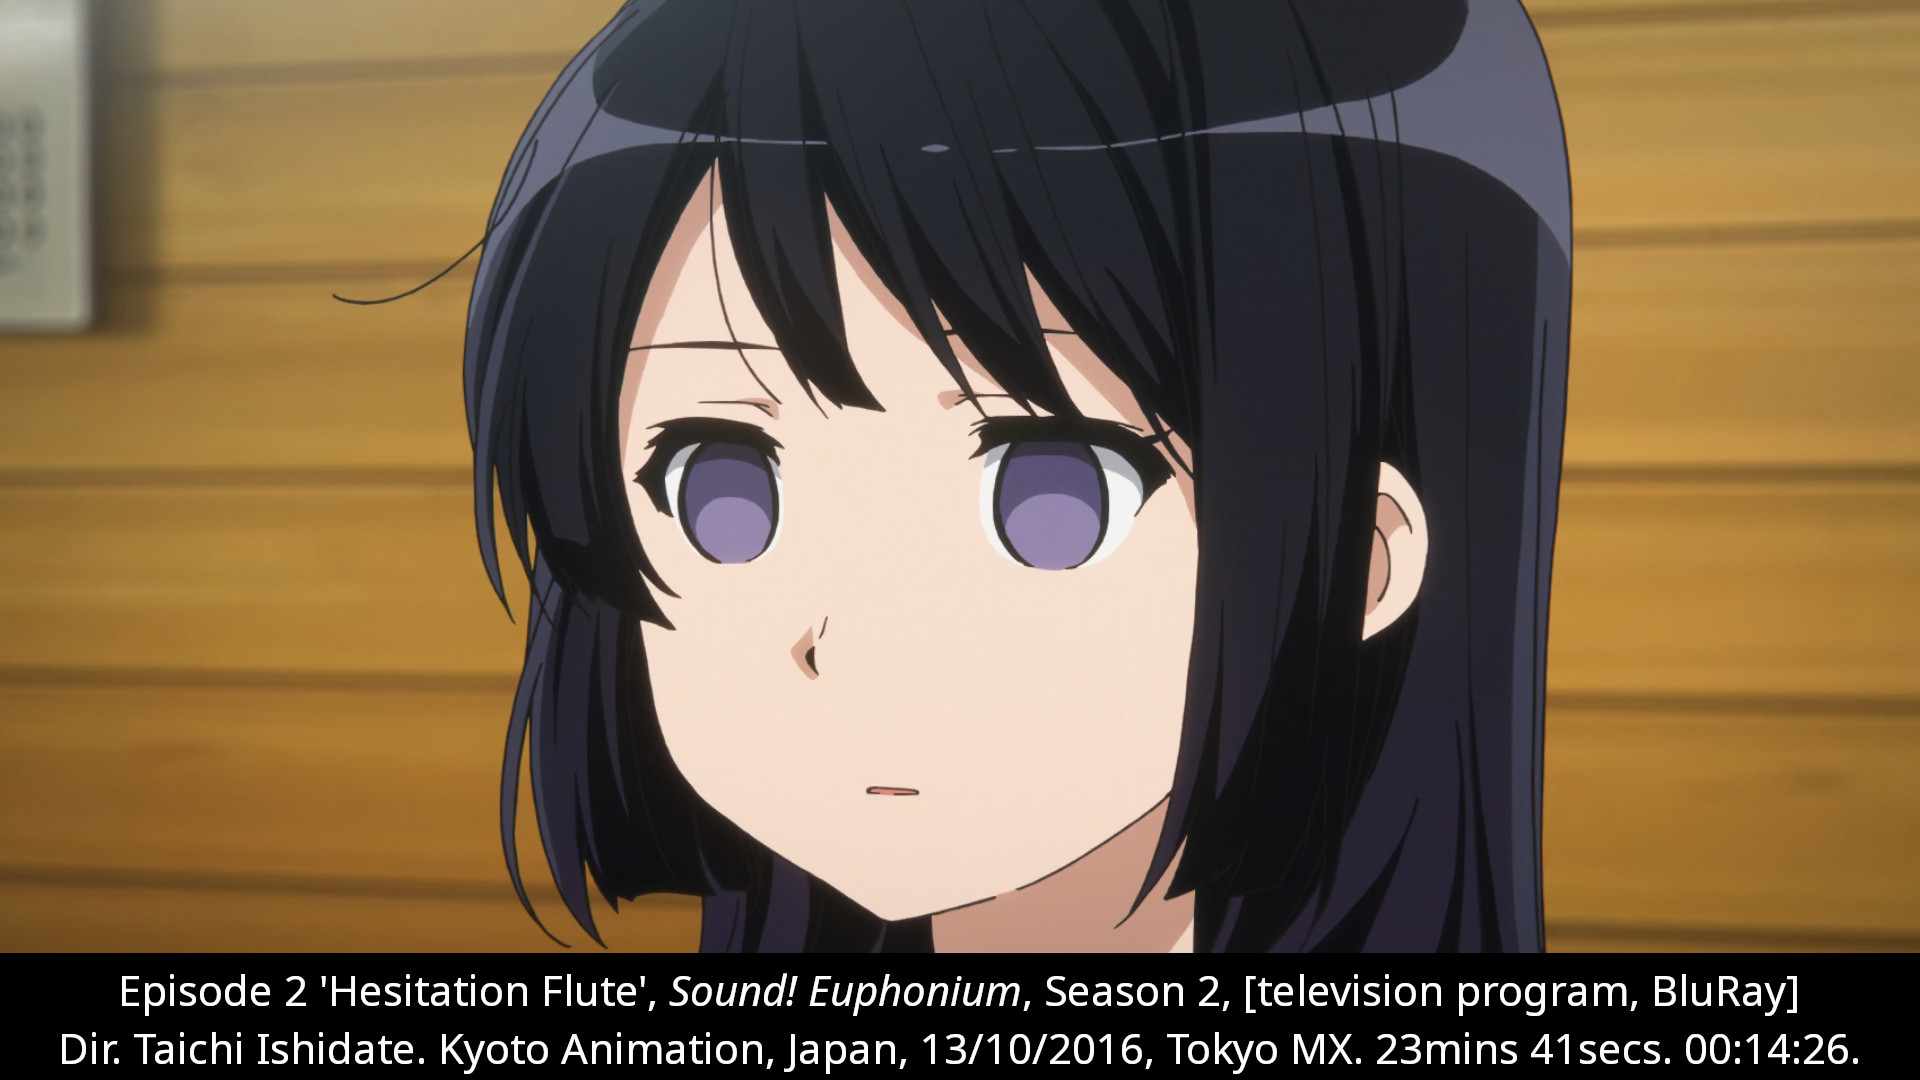
\includegraphics[width=\paperwidth, height=\paperheight]{images/00:14:26 Reina FishEyes Saison 2 Episode 2.jpg}
  \end{columns}
\end{frame}
% Episode 2 'Hesitation Flute', \emph{Sound! Euphonium}, Saison 2, [television program, BluRay] Dir. Taichi Ishidate. Kyoto Animation, Japan, 13/10/2016, Tokyo MX. 23mins 41secs. 00:14:26.
% using the http://bufvc.ac.uk/wp-content/media/2013/03/BUFVC-AV-Citation-ONLINE.pdf referencing guide
\begin{frame}[fragile]{PERL string incremented to float explanation}
    \note[item]{
        We arrive at one point to the string "5d9" which when incremented gives use "5e0",
        which is a number written in scientific notation which gets converted to float
    }
    \begin{minted}[startinline]{php}
$s = "5d9";
var_dump(++$s); // string(3) "5e0"
var_dump(++$s); // float(6)
    \end{minted}
\end{frame}

\begin{frame}[fragile]{Array offsets}
    \note{Array offsets can either be integers or strings}
    \begin{onlyenv}<1>
        \begin{minted}[startinline]{php}
$a = [];
$a[5] = "Fifth key";
$a["string key"] = "Usual string key";
$a["2"] = "Integer string key";
$a["007"] = "Numeric string key";
$a[""] = "Empty key";

var_dump($a);
        \end{minted}
    \end{onlyenv}
    \begin{onlyenv}<2>
        \begin{minted}[startinline]{php}
array(5) {
  [5]=>
  string(9) "Fifth key"
  ["string key"]=>
  string(16) "Usual string key"
  [2]=>
  string(18) "Integer string key"
  ["007"]=>
  string(18) "Numeric string key"
  [""]=>
  string(9) "Empty key"
}
        \end{minted}
    \end{onlyenv}
\end{frame}
\begin{frame}[fragile]{Array offset type juggling}
    \begin{onlyenv}<1>
        \begin{minted}[startinline]{php}
$a = [];
$a[null] = "null";
$a[false] = false;
$a[true] = true;

var_dump($a);
        \end{minted}
    \end{onlyenv}
    \begin{onlyenv}<2>
        \begin{minted}[startinline,breaklines]{php}
array(3) {
  [""]=>
  string(4) "null"
  [0]=>
  bool(false)
  [1]=>
  bool(true)
}
        \end{minted}
    \end{onlyenv}
    \begin{onlyenv}<3>
        \begin{minted}[startinline]{php}
$a = [];
$a[15.5] = 15.5;
$a["15.5"] = "15.5";

var_dump($a);
        \end{minted}
    \end{onlyenv}
    \begin{onlyenv}<4>
        \begin{minted}[startinline,breaklines]{php}
Deprecated: Implicit conversion from float 15.5 to int loses precision
array(2) {
  [15]=>
  float(15.5)
  ["15.5"]=>
  string(4) "15.5"
}
        \end{minted}
    \end{onlyenv}
    \begin{onlyenv}<5>
        \begin{minted}[startinline,breaklines]{php}
$a[STDERR] = "Resource";
var_dump($a);
// Warning: Resource ID#3 used as offset, casting to integer (3)
array(1) {
  [3]=>
  string(8) "Resource"
}

$a[[]] = "Array";
// TypeError: Illegal offset type
        \end{minted}
    \end{onlyenv}
    \begin{onlyenv}<6>
        \begin{minted}[startinline,breaklines]{php}
$o = new stdClass();
$a[$o] = "Object";
// TypeError: Illegal offset type

class Stringy {
    public function __toString() { return "foo"; }
}
$stringable = new Stringy();
$a[$stringable] = "Stringable";
// TypeError: Illegal offset type
        \end{minted}
    \end{onlyenv}
\end{frame}
\begin{frame}[fragile]{Unset Array Offsets}
    \begin{onlyenv}<1>
        \begin{minted}[startinline,breaklines]{php}
unset($a[null]);
unset($a[false]);
unset($a[true]);
unset($a[15.5]);
Deprecated: Implicit conversion from float 15.5 to int loses precision
unset($a[STDERR]);
Warning: Resource ID#3 used as offset, casting to integer (3)
        \end{minted}
    \end{onlyenv}
    \begin{onlyenv}<2>
        \begin{minted}[startinline]{php}
unset($a[[]]);
// TypeError: Illegal offset type

unset($a[$o]);
// TypeError: Illegal offset type
        \end{minted}
    \end{onlyenv}
\end{frame}
\begin{frame}[fragile]{\texttt{empty}/\texttt{isset} Array Offsets}
    \begin{onlyenv}<1>
        \begin{minted}[startinline,breaklines]{php}
var_dump(empty($a[null]));   // bool(false)
var_dump(empty($a[false]));  // bool(true)
var_dump(empty($a[true]));   // bool(false)
var_dump(empty($a[15.5]));   // bool(false)
// Deprecated: Implicit conversion from float 15.5 to int loses precision
var_dump(empty($a[STDERR])); // bool(false)
// Warning: Resource ID#3 used as offset, casting to integer (3)
        \end{minted}
    \end{onlyenv}
    \begin{onlyenv}<2>
        \begin{minted}[startinline]{php}
empty($a[[]]);
// TypeError: Illegal offset type

empty($a[$o]);
// TypeError: Illegal offset type
        \end{minted}
    \end{onlyenv}
    \begin{onlyenv}<3>
        \begin{minted}[startinline,breaklines]{php}
var_dump(isset($a[null]));   // bool(true)
var_dump(isset($a[false]));  // bool(true)
var_dump(isset($a[true]));   // bool(true)
var_dump(isset($a[15.5]));   // bool(true)
// Deprecated: Implicit conversion from float 15.5 to int loses precision
var_dump(isset($a[STDERR])); // bool(true)
// Warning: Resource ID#3 used as offset, casting to integer (3)
        \end{minted}
    \end{onlyenv}
    \begin{onlyenv}<4>
        \begin{minted}[startinline]{php}
isset($a[[]]);
// TypeError: Illegal offset type

isset($a[$o]);
// TypeError: Illegal offset type
        \end{minted}
    \end{onlyenv}
    \begin{onlyenv}<5>
        \begin{minted}[startinline,breaklines]{php}
var_dump($a[null]  ?? 'default');  // string(4) "null"
var_dump($a[false] ?? 'default');  // bool(false)
var_dump($a[true]  ?? 'default');  // bool(true)
var_dump($a[15.5]  ?? 'default');  // float(15.5)
// Deprecated: Implicit conversion from float 15.5 to int loses precision
var_dump($a[STDERR] ?? 'default'); // string(8) "Resource"
// Warning: Resource ID#3 used as offset, casting to integer (3)
        \end{minted}
    \end{onlyenv}
    \begin{onlyenv}<6>
        \begin{minted}[startinline]{php}
var_dump($a[[]] ?? 'default');
// TypeError: Illegal offset type

var_dump($a[$o] ?? 'default');
// TypeError: Illegal offset type
        \end{minted}
    \end{onlyenv}
\end{frame}

\begin{frame}[fragile]{String offsets}
    \note{String offsets must be integers}
    \begin{onlyenv}<1-2>
        \begin{minted}[startinline]{php}
$s = "abcdefghijklmnopqrstuvwxyz";
var_dump($s[6]);     // string(1) "g"
        \end{minted}
        \vfill
    \end{onlyenv}
    \begin{onlyenv}<2>
        \begin{minted}[startinline]{php}
var_dump($s[null]);  // string(1) "a"
// Warning: String offset cast occurred

var_dump($s[false]); // string(1) "a"
// Warning: String offset cast occurred

var_dump($s[true]);  // string(1) "b"
// Warning: String offset cast occurred
        \end{minted}
    \end{onlyenv}
    \begin{onlyenv}<3>
        \begin{minted}[startinline]{php}
var_dump($s[8.0]); // string(1) "i"
// Warning: String offset cast occurred

var_dump($s[8.6]); // string(1) "i"
// Warning: String offset cast occurred
        \end{minted}
    \end{onlyenv}
    \begin{onlyenv}<4>
        \begin{minted}[startinline,breaklines]{php}
var_dump($s["2"]);    // string(1) "c"
var_dump($s["007"]);  // string(1) "h"
var_dump($s["19.0"]);
// TypeError: Cannot access offset of type string on string
var_dump($s["19.6"]);
// TypeError: Cannot access offset of type string on string
var_dump($s["key"]);
// TypeError: Cannot access offset of type string on string
        \end{minted}
    \end{onlyenv}
    \begin{onlyenv}<5>
        \begin{minted}[startinline,breaklines]{php}
var_dump($s[[]]);
// TypeError: Cannot access offset of type array on string
var_dump($s[STDERR]);
// TypeError: Cannot access offset of type resource on string
$o = new stdClass();
var_dump($s[$o]);
// TypeError: Cannot access offset of type stdClass on string
        \end{minted}
    \end{onlyenv}
\end{frame}
\begin{frame}[fragile]{Unset String Offsets}
    \begin{minted}[startinline]{php}
unset($s[6]);
// Error: Cannot unset string offsets
    \end{minted}
    \pause
    \begin{minted}[startinline]{php}
unset($s["a"]["b"]);
// TypeError: Cannot access offset of type string on string
    \end{minted}
\end{frame}

\begin{frame}[fragile]{\texttt{empty}/\texttt{isset} String Offsets}
    \begin{onlyenv}<1>
        \begin{minted}[startinline,breaklines]{php}
var_dump(empty($s[6]));     // bool(false)
var_dump(empty($s[null]));  // bool(false)
var_dump(empty($s[false])); // bool(false)
var_dump(empty($s[true]));  // bool(false)
var_dump(empty($s[8.0]));   // bool(false)
var_dump(empty($s[8.6]));   // bool(false)
// Deprecated: Implicit conversion from float 8.6 to int loses precision
        \end{minted}
    \end{onlyenv}
    \begin{onlyenv}<2>
        \begin{minted}[startinline]{php}
var_dump(empty($s["2"]));    // bool(false)
var_dump(empty($s["007"]));  // bool(false)
var_dump(empty($s["19.0"])); // bool(true)
var_dump(empty($s["19.6"])); // bool(true)
var_dump(empty($s["key"]));  // bool(true)
var_dump(empty($s[[]]));     // bool(true)
var_dump(empty($s[STDERR])); // bool(true)
var_dump(empty($s[$o]));     // bool(true)
        \end{minted}
    \end{onlyenv}
    \begin{onlyenv}<3>
        \begin{minted}[startinline,breaklines]{php}
var_dump(isset($s[6]));     // bool(true)
var_dump(isset($s[null]));  // bool(true)
var_dump(isset($s[false])); // bool(true)
var_dump(isset($s[true]));  // bool(true)
var_dump(isset($s[8.0]));   // bool(true)
var_dump(isset($s[8.6]));   // bool(true)
// Deprecated: Implicit conversion from float 8.6 to int loses precision
        \end{minted}
    \end{onlyenv}
    \begin{onlyenv}<4>
        \begin{minted}[startinline]{php}
var_dump(isset($s["2"]));    // bool(true)
var_dump(isset($s["007"]));  // bool(true)
var_dump(isset($s["19.0"])); // bool(false)
var_dump(isset($s["19.6"])); // bool(false)
var_dump(isset($s["key"]));  // bool(false)
var_dump(isset($s[[]]));     // bool(false)
var_dump(isset($s[STDERR])); // bool(false)
var_dump(isset($s[$o]));     // bool(false)
        \end{minted}
    \end{onlyenv}
    \begin{onlyenv}<5>
        \begin{minted}[startinline]{php}
var_dump($s[6] ?? 'default');     // string(1) "g"
var_dump($s[null] ?? 'default');  // string(1) "a"
var_dump($s[false] ?? 'default'); // string(1) "a"
var_dump($s[true] ?? 'default');  // string(1) "b"
var_dump($s[8.0] ?? 'default');   // string(1) "i"
var_dump($s[8.6] ?? 'default');   // string(1) "i"
        \end{minted}
    \end{onlyenv}
    \begin{onlyenv}<6>
        \begin{minted}[startinline,breaklines]{php}
var_dump($s["2"] ?? 'default');    // string(1) "c"
var_dump($s["007"] ?? 'default');  // string(1) "h"
var_dump($s["19.0"] ?? 'default'); // string(7) "default"
var_dump($s["19.6"] ?? 'default'); // string(7) "default"
var_dump($s["key"] ?? 'default');  // string(7) "default"
        \end{minted}
    \end{onlyenv}
    \begin{onlyenv}<7>
        \begin{minted}[startinline,breaklines]{php}
var_dump($s[STDERR] ?? 'default');
// TypeError: Cannot access offset of type resource on string
var_dump($s[[]] ?? 'default');
// TypeError: Cannot access offset of type array on string
var_dump($s[$o] ?? 'default');
// TypeError: Cannot access offset of type object on string
        \end{minted}
    \end{onlyenv}
\end{frame}

\begin{frame}[plain]
  \begin{columns}[c]
    \column{\paperwidth}
    
\includegraphics[width=\paperwidth, height=\paperheight]{images/00:02:56 Yuuko face Saison 2 Episode 13.jpg}
  \end{columns}
\end{frame}
% Episode 13 'Early-Spring Epilogue', \emph{Sound! Euphonium}, Saison 2, [television program, BluRay] Dirs. Tatsuya Ishihara, Naoko Yamada, Eisaku Kawanami. Kyoto Animation, Japan, 28/12/2016, Tokyo MX. 23mins 41secs. 00:02:56.
% using the http://bufvc.ac.uk/wp-content/media/2013/03/BUFVC-AV-Citation-ONLINE.pdf referencing guide

\begin{frame}[fragile]{\texttt{exit} construct}
    \texttt{exit} accepts either an \type{int} or \type{string}
    \note{Using 3v4l.org we get the following}
    \begin{minted}[startinline]{php}
exit(10);
// Process exited with code 10.
    \end{minted}
    \begin{minted}[startinline]{php}
exit("Programm exit");
// Programm exit
    \end{minted}
\end{frame}
\begin{frame}[fragile]{\texttt{exit} construct}
    If the value is not an \type{int} then \texttt{exit} will interpret it as \type{string}
    \begin{onlyenv}<1>
        \begin{minted}[startinline]{php}
exit(null);
//
        \end{minted}
        \begin{minted}[startinline]{php}
exit(false);
//
        \end{minted}
        \begin{minted}[startinline]{php}
exit(true);
// 1
        \end{minted}
        \begin{minted}[startinline]{php}
exit(15.0);
// 15
        \end{minted}
    \end{onlyenv}
    \begin{onlyenv}<2>
        \begin{minted}[startinline]{php}
exit([]);
// Warning: Array to string conversion in %s on line %d
// Array
        \end{minted}
        \begin{minted}[startinline]{php}
$r = STDERR;
exit($r);
// Resource id #3
        \end{minted}
    \end{onlyenv}
    \begin{onlyenv}<3>
        \begin{minted}[startinline]{php}
$o = new stdClass;
try {
    exit($o);
} catch (\Error $e) {
    echo $e::class, PHP_EOL, "I've escaped the exit";
}
// Error
// I've escaped the exit
        \end{minted}
    \end{onlyenv}
\end{frame}


\begin{frame}{Which type juggling contexts does \texttt{strict\_types} affect?}
    \note[item]{Be sorry about the cursed knowledge you are going to inflict}
    \begin{enumerate}
        \item String
        \item Integral and String
        \item Numeric
        \item Logical
        \item Comparative
        \item \alert<2>{Function}
        \item Increment/Decrement operators
        \item Array offsets
        \item String offsets
        \item \texttt{exit} construct
    \end{enumerate}
\end{frame}

\begin{frame}{What does \texttt{strict\_types} do?}
    Only enabled in PHP scripts that use \texttt{declare(strict\_types=1);}
    
    Disables coercion of scalar types in the following cases \alert{only}:
    \begin{itemize}
        \item Arguments passed to function calls made in userland
        \item Return value for user defined functions
        \item Value assignment to a typed property
    \end{itemize}
\end{frame}
\begin{frame}[fragile]{\texttt{strict\_types}}
    \texttt{strict\_types} does \alert{not} change the behaviour of:

    \begin{itemize}
        \begin{onlyenv}<1>
            \vfill
        \end{onlyenv}
        \begin{onlyenv}<2>
            \item Binary operations:
            \begin{minted}[startinline]{php}
declare(strict_types=1);
var_dump(10 + "45"); // int(55)
var_dump(true . " hello"); // string(7) "1 hello"
            \end{minted}
            \vfill
        \end{onlyenv}
        \begin{onlyenv}<3>
            \item Comparison operations:
            \begin{minted}[startinline]{php}
declare(strict_types=1);
var_dump("1" == "01"); // bool(true)
var_dump(014 == "14"); // bool(false)
var_dump(14 == "014"); // bool(true)
            \end{minted}
            \vfill
        \end{onlyenv}
        \begin{onlyenv}<4>
            \item \texttt{exit} construct:
            \begin{minted}[startinline]{php}
declare(strict_types=1);
exit(true);
// 1
            \end{minted}
            \vfill
        \end{onlyenv}
        \begin{onlyenv}<5>
            \item Scalar type coercion for functions called by the engine:
            \begin{minted}[startinline,fontsize=\footnotesize,breaklines]{php}
declare(strict_types=1);
$f = fn (int $i): bool => (bool) ($i % 2);
$a = ['1', '2', 3, 4, '5.0', '6.0'];
var_dump(array_filter($a, $f));
/* array(3) {
  [0]=>
  string(1) "1"
  [2]=>
  int(3)
  [4]=>
  string(3) "5.0"
} */
            \end{minted}
        \end{onlyenv}
    \end{itemize}
\end{frame}

\begin{frame}{Hot take}
    The \texttt{strict\_types} declare was a \alert{mistake}.
\end{frame}

{\setbeamercolor{palette primary}{fg=AFUP_text, bg=AFUP}
\begin{frame}[standout]
    Thank you!
    \begin{description}[Mastodon:]
        \item[GitHub:] Girgias
        \item[Site:] \url{https://gpb.moe}
        \item[Mastodon:] @Girgias@phpc.social
        \item[Twitter:] @Girgias
    \end{description}
\end{frame}
}
\appendix

\begin{frame}[allowframebreaks]{References}
  %\bibliography{type_talk}
  %\bibliographystyle{abbrv}
  \printbibliography
\end{frame}

\end{document}
